\documentclass[a4paper,12pt]{article}

% --- Поддержка русского языка ---
\usepackage[T1, T2A]{fontenc}    % Кодировка шрифтов
\usepackage[utf8]{inputenc}
\usepackage{unicode-math}

\usepackage{polyglossia} % Замена babel для XeLaTeX
\setmainlanguage{russian}
\setotherlanguage{english}

% 1. Основной шрифт (с засечками), поддерживающий кириллицу
\setmainfont{Libertinus Serif} % Или Times New Roman, если Libertinus глючит

% 2. Шрифт без засечек (опционально)
\setsansfont{Libertinus Sans}

% Подключаем JetBrains Mono для моноширинного текста
\setmonofont{JetBrains Mono}[
    Scale=0.3, % JB Mono крупноват, лучше чуть уменьшить
    Contextuals=Alternate % Включает лигатуры, если они нужны
]

% 4. Явное указание шрифта для кириллицы (решает вашу ошибку в polyglossia)
\newfontfamily{\cyrillicfont}{Libertinus Serif}
\newfontfamily{\cyrillicfonttt}{JetBrains Mono}

\usepackage{tikz}
\usetikzlibrary{arrows.meta,positioning,fit,calc}
\usepackage{xparse}
\usepackage{cellspace}
\setlength\cellspacetoplimit{4pt}
\setlength\cellspacebottomlimit{4pt}

\usepackage{csquotes}

% --- Поля и форматирование ---
\usepackage[left=2cm,right=2cm,top=2cm,bottom=2cm]{geometry} % Поля
\usepackage{indentfirst} % Красная строка в первом абзаце
\usepackage[scaled]{beramono}
\usepackage{listings}

\lstset{
    basicstyle=\ttfamily\small,
    columns=flexible,          % Убирает лишние пробелы между буквами, код станет плотнее
    keepspaces=true,
    aboveskip=1em,             % Добавит нормальный отступ сверху
    belowskip=1em,             % И снизу
    xleftmargin=1.5em,         % Код визуально «втянется» внутрь текста
    basicstyle=\ttfamily\small\color{black!85},
}

% --- Математика и графика ---
\usepackage{graphicx} % Для вставки картинок

\usepackage{fontspec}

\setmainfont{Libertinus Serif}
\setsansfont{Libertinus Sans}
\setmonofont{Libertinus Mono}
\setmathfont{Libertinus Math}

\tikzset{
    recordbox/.style={
        draw,
        inner xsep=6pt,
        inner ysep=4pt,
        outer sep=0pt,
        align=center
    },
    recorddot/.style={
        draw,
        inner sep=2pt,
        minimum width=1.2em,
        outer sep=0pt,
        align=center
    }
}
\makeatletter
\pgfkeys{/tikz/minimumheight/.code=\pgfkeysalso{/tikz/minimum height=#1}}
\pgfkeys{/tikz/minimumwidth/.code=\pgfkeysalso{/tikz/minimum width=#1}}
\makeatother

% --- Информация о статье ---
\title{Архитектура объектового хранилища Apogee.}
\author{Денис Черемисов}
\date{\today}

\begin{document}

    \maketitle

    \begin{abstract}
        Данная статья содержит описание архитектуры объектового хранилища ориентированного на масштабирование, высокую локальную и глобальную производительность и качественную диагностируемость
        за счёт простой схемы взаимодействия компонентов, каждый из которых четко изолирован в рамках своего домена ответственности.
    \end{abstract}

    \newpage
    \tableofcontents
    \newpage  % необязательно


    \section{Определения.}

    Система делится на следующие компоненты:

    \begin{itemize}
        \item Координаторы без состояния.

        \item Холод, делящийся на холодные узлы:
        \begin{itemize}
            \item RAFT аллокатор выделения кортежей и \textit{страйпов} на них.
            \item Кортежи дисков обслуживаемые аллокатором.
        \end{itemize}

        \item Жара, она представлена узлами из трёх машин в идентичной конфигурации.Возможны несколько вариантов в зависимости от требований к цене и производительности.

        \item WAL, распределённый WAL, пока проще всего реализовать с помощью брокера и KV хранилища с персистетностью и гарантиями. Например, на основе Nats + JetStream, который и брокер и KV.

        \item Метаданные:
        \begin{itemize}
            \item Записи Records с метаданными записей.
            \item Фрагменты Fragments с метаданными фрагментов включащих поля поддержки дедупликации.
            \item Коллекция Links для связи Records и Fragments.
            \item Containers для описания физического размещения контейнеров с фрагментами: контейнер может быть \enquote{запечатан} в страйпе холодного слоя либо пока лежать на буфере горячего слоя.
            \item Tuples для связи кортежей холодного слоя с дисками
        \end{itemize}
    \end{itemize}

    \newpage


    \section{Физическое устройство системы.}

    \subsection{Слой горячего хранения.}

    Здесь я предлагаю три разных подхода, отличающихся экзотичностью железа и ценой. Во всех случаях в горячем слое мы используем максимальную степень избыточности.
    Т.к. на этом этапе проще всего работать от \enquote{наибольшего знаменателя}, т.е. использовать схему \times 3, а уже в холодном хранилище понижать степень избыточности.
    Т.е. когда мы говорим о \enquote{горячем узле} мы имеем в виду три узла, каждый из которых хранит копию данных. И соответствующие накопители на машинах должны быть
    эквивалентными с точки зрения аппаратного LBA и объёма.

    В любом из режимов диск $D_i$ представляется в следующем виде:

    \begin{gather*}
        D_i = \left(B_{i1}, B_{i2}, \dots, B_{im}\right)\\
        |B_{i1}| = |B_{i2}| = \dots = |B_{im}| = 64\text{MiB}\\
    \end{gather*}
    Блоки $B_{ij}$ называются \textit{буферами}.

    \subsubsection{Максимальная производительность.}

    Аппаратные требования:

    \begin{itemize}
        \item Один или несколько NVMe SSD.
        \item Плашка/плашки NVDIMM (дешевле чем Optane при схожих гарантиях).
    \end{itemize}

    В этом режиме мы используем NVMe SSD. Один, два, три. Больше вряд ли имеет смысл, т.к. три накопителя сожрут любую сеть, а NVMe на PCI-e x5 сожрет в одиночку.


    \smallskip
    И для каждого диска $D_i$ на NVDIMM плашках выделяется область памяти $M_i$, которая так же делится на равные фрагменты $M_{ij}$, где $j = 1, 2, \dots, m$:

    \begin{gather*}
        M_i = \left(M_{i1}, M_{i2}, \dots, M_{im}\right)\\
        |M_{i1}| = |M_{i2}| = \dots = |M_{im}|\\
    \end{gather*}

    \begin{center}
        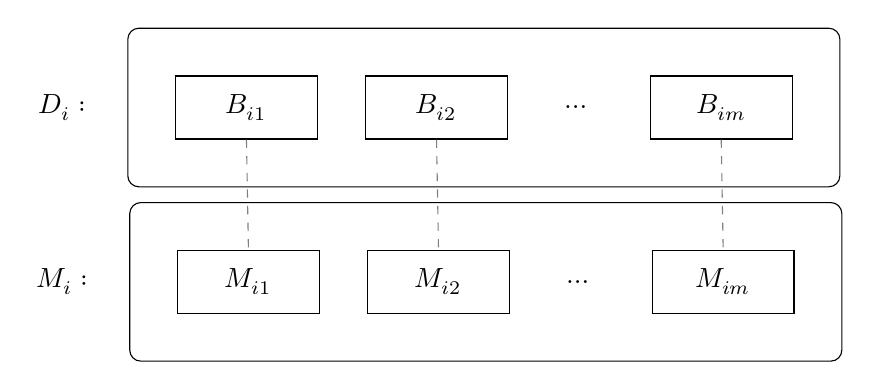
\begin{tikzpicture}[
            block/.style={
                draw,
                minimum width=18mm,
                minimum height=8mm,
                align=center
            },
            rowlabel/.style={
                align=right,
                minimum height=8mm
            },
            container/.style={
                draw,
                rounded corners,
                inner sep=6mm
            },
            node distance=6mm
        ]

% --- Row label for D_i ---
            \node[rowlabel] (Dl) {$D_i:$};

% --- Blocks B_ij (disk) ---
            \node[block, right=10mm of Dl] (B1) {$B_{i1}$};
            \node[block, right=of B1] (B2) {$B_{i2}$};
            \node[right=of B2] (Bdots) {$\dots$};
            \node[block, right=of Bdots] (Bm) {$B_{im}$};

            \node[
                container,
                fit=(B1)(B2)(Bdots)(Bm)
            ] (Drow) {};

% --- Row label for M_i ---
            \node[rowlabel, below=14mm of Dl] (Ml) {$M_i:$};

% --- Fragments M_ij (memory) ---
            \node[block, right=10mm of Ml] (M1) {$M_{i1}$};
            \node[block, right=of M1] (M2) {$M_{i2}$};
            \node[right=of M2] (Mdots) {$\dots$};
            \node[block, right=of Mdots] (Mm) {$M_{im}$};

            \node[
                container,
                fit=(M1)(M2)(Mdots)(Mm)
            ] (Mrow) {};

% --- Alignment guides ---
            \foreach \b/\m in {B1/M1,B2/M2,Bm/Mm} {
                \draw[dashed, gray] (\b.south) -- (\m.north);
            }
        \end{tikzpicture}
    \end{center}
    Размер фрагментов $M_{ij}$ определяется исходя из физического размера блока на дисках.
    Каждый $M_{ij}$ хранит:

    \begin{itemize}
        \item метаданные контейнера заполняемого (или заполненного) в буфере $B_{ij}$.
        \item буфер в смысле буферизованного IO для незаполненных при записи LBA.
    \end{itemize}
    При последующих записях этот буфер будет заполнен до конца и улетит в хвост $B_{ij}$.

    Обратим вниманием на выбор буферов для записи. Мы должны смещаться от начала диска до его конца при выборе. Т.е. все блоки $B_{ij}$ будут заполняться почти последовательно. Это обеспечит
    равномерный износ накопителя. И при неудавшейся записи мы ни в коем случае не должны пытаться вновь писать в тот же блок. Потому что это будет попытка перезаписи и это будет напрасным
    износом диска. Просто проскакиваем область LBA которая должна была содержать фрагмент и всё. Т.е. фундаментально придерживаемся append-семантики.

    \smallskip
    Такой подход позволяет обслуживать сотни видео-стримов в высоком разрешении.

    \subsubsection{Высокая производительность.}

    Аналогично предыдущему пункту, но без NVDIMM. В этом случае метаданные буферов будут храниться в какой-либо базке, а вот упаковки в LBA не будет. Т.е. если запись не поместилась
    в блок накопителя целиком, то остаток блока заполняется нулями и следующая запись начинается с начала следующего блока.

    В целом, такой подход будет обеспечивать достаточно высокую производительность, хотя уступающую прыдущему варианту. Но для видео-стримов подходить будет хуже, придётся заморачиваться с
    буферизацией по LBA на координаторах. Что явно нехорошо, т.к. это будет требовать знания кишок жары.

    \subsubsection{Вариант для дешёвых on-premise решений.}

    Диск как кольцевой буфер.
    \smallskip

    Здесь мы вообще не заморачиваемся более-менее плотной упаковкой буферов и если записываемый фрагмент выходит за границы буфера, то мы сразу запечатываем буфер и готовим его
    к перевозу в холод, а фрагмент пишем уже на следующий. Такой подход противопоказан стримам, т.е. такая жара подходит только для всяких хранилищ документов. Но зато она дешёвая и может
    быть реализована на любом железе, даже на HDD.

    \subsection{Слой холодного хранения.}

    Он разбивается на холодные узлы и каждый узел это пара:
    \begin{itemize}
        \item RAFT-аллокатор.
        \item Набор кортежей дисков.
    \end{itemize}

    Кортеж $T$ представляет собой набор дисков
    \[T=\left( D_1, D_2, \dots, D_N \right)\]
    Сами диски представляются как наборы блоков одинакового между собою размера:
    \[D_i = \left( C_{i1}, C_{i2}, \dots, C_{iM} \right)\]
    \textit{Страйпом} $S_j$ в кортеже $T$ называется набор блоков с индексом $j$ набранных со всех дисков кортежа:
    \[S_j = \left( C_{1j}, C_{2j}, \dots, C_{Nj} \right)\]

    Задачей RAFT-аллокатора является поиск свободных страйпов в обслуживаемых кортежах. Т.е. вначале он выбирает один из кортежей и затем ищет свободный страйп.
    Учёт свободный-несвободный ведётся с помощью \textit{битмапа} кортежа, где каждому страйпу сопоставлен бит, имеющий значение 1 для занятых и 0 для свободных
    страйпов:

    \begin{center}
        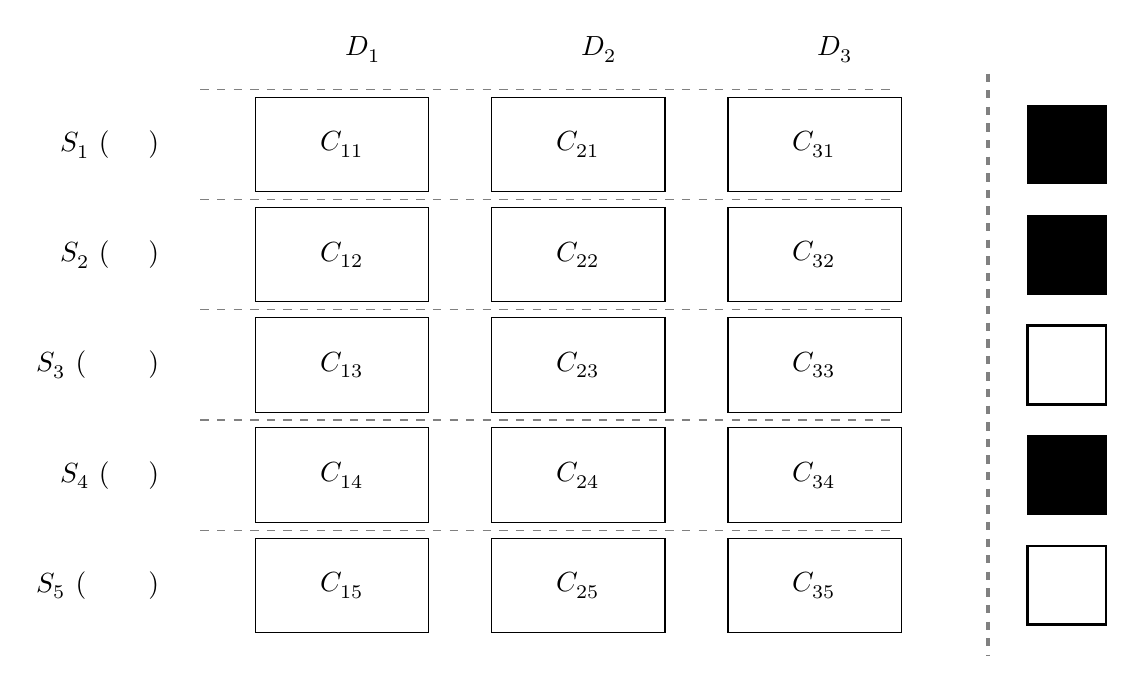
\begin{tikzpicture}[
            block/.style={
                draw,
                minimum width=2.2cm,
                minimum height=1.2cm,
                align=center
            },
            stripe/.style={
                dashed,
                gray
            },
            vsep/.style={
                dashed,
                very thick,
                gray
            },
            bitone/.style={
                draw,
                fill=black,
                minimum width=1.0cm,
                minimum height=1.0cm
            },
            bitzero/.style={
                draw,
                fill=white,
                line width=1pt,
                minimum width=1.0cm,
                minimum height=1.0cm
            }
        ]

% Parameters
            \def\ndisks{3}
            \def\nstripes{5}

% --- Bitmap definition: 1 = occupied, 0 = free ---
% Put exactly \nstripes values here, in order S1..S5:
            \def\bitmap{1,1,0,1,0}

% Layout parameters
            \def\xDiskStep{3}
            \def\yStripeStep{1.4}
            \def\xLabel{0.8}
            \def\xStripeLineL{1.2}
            \def\xStripeLineR{10}

% Bitmap column x positions
            \def\xSep{11.2}     % vertical separator x
            \def\xBmp{12.2}     % bitmap squares x

% Disk labels
            \foreach \i in {1,...,\ndisks} {
                \node at (\i*\xDiskStep, -0.2) {\textbf{Диск $D_{\i}$}};
            }

% Blocks C_ij
            \foreach \i in {1,...,\ndisks} {
                \foreach \j in {1,...,\nstripes} {
                    \node[block] (c\i\j) at (\i*\xDiskStep, -\j*\yStripeStep) {$C_{\i\j}$};
                }
            }

% Stripe separators, labels, and bitmap squares
            \foreach[count=\j from 1] \b in \bitmap {

            % horizontal dashed stripe line
                \draw[stripe] (\xStripeLineL, -\j*\yStripeStep+0.7) -- (\xStripeLineR, -\j*\yStripeStep+0.7);

            % stripe label: S_j (occupied/free)
                \ifnum
                    \b=1
                    \node[anchor=east] at (\xLabel, -\j*\yStripeStep) {$S_{\j}$ (занят)};
                \else
                    \node[anchor=east] at (\xLabel, -\j*\yStripeStep) {$S_{\j}$ (свободен)};
                \fi

            % bitmap square
                \ifnum
                    \b=1
                    \node[bitone]  at (\xBmp, -\j*\yStripeStep) {};
                \else
                    \node[bitzero] at (\xBmp, -\j*\yStripeStep) {};
                \fi
            }

% Bitmap title
            \node[anchor=west] at (\xBmp-0.6, -0.2) {\textbf{Битмап}};

% Vertical dashed separator (covers all stripes)
            \draw[vsep]
            (\xSep, -1*\yStripeStep+0.9) -- (\xSep, -\nstripes*\yStripeStep-0.9);

        \end{tikzpicture}
    \end{center}
    Выделение страйпа производится в два шага:

    \begin{enumerate}
        \item Lease страйпа.
        \item Подтверждение занятия страйпа (Commit) или отмена занятия (Release).
    \end{enumerate}

    Release производится автоматически по TTL, если от координатора ведущего миграцию не было никакого сигнала в течении $\Delta$ секунд. Таким образом, для перемещения 64МиБ данных у нас
    проводятся 2 RAFT-операции. Это 64 RAFT-операции в секунду на проводку потока данных в обе объёме 2ГиБ в секунду. Это ничтожно мало, тем более в условиях когда задержки нас не особо
    волнуют т.к. это фоновый процесс.

    \subsection{Выбор кортежа.}

    При выборе кортежа важно склоняться к выбору наименее заполненных и не слишком сильно загруженных в данный момент. Следующий алгоритм должен
    быть рабочим.

    Есть некоторый параметр – натуральное число $N$. Кортежи хранятся в структуре
    \begin{lstlisting}
tuples = RBTree[FreeStripes, LinkedList[Tuple]]
    \end{lstlisting}
    Т.е. кортежи сгрупированны по количеству доступных для записи страйпов в них и упорядочены по количеству этих страйпов. Выбор страйпа под
    запись осуществляется следующим образом:
    \begin{enumerate}
        \item Выбираем случайный $K$ из $\left[ 0, N \right)$.
        \item Берём $K$-ый кортеж из структуры и запускем там процесс записи данных.
        \item После подтверждения записи, изымаем кортеж из связного списка с данным весом и переносим в конец списка с весом ниже.
    \end{enumerate}
    Можно пропускать сильно нагруженные в данный момент кортежи, вообще не учитывая их, в поиске $K$-го. Это приведёт
    к увеличению сложности поиска, но мы говорим о всего 32 таких операциях на 2Гб/с.

    \subsection{Мета}

    В качестве БД для хранения метаданных лучше всего подходит TiKV: практически неограниченное горизонтальное масштабирование, высокая
    производительность, особенно в rawkv режиме.

    \subsubsection{Records}

    \begin{tabular}{|Sl|Sc|Sc|Sr|}
        \hline
        record.id & single & fragment.id & $\dots$ \\
        \hline
    \end{tabular}

    \bigskip

    \begin{tabular}{|Sl|Sc|Sc|Sr|}
        \hline
        record.id & multi & no\_of\_fragments & $\dots$ \\
        \hline
    \end{tabular}

    \bigskip
    Хранит метаданные записей. Здесь мы в случае одного фрагмента в записи храним ссылку на него прямо в records, чтобы избежать
    избыточного хранения данных. В случае хранилища мелкодокументов получим полуторакратное уменьшение числа записей в метаслое: не будет
    записей в Links.

    \subsubsection{Fragments}

    \begin{tabular}{|Sl|Sc|Sc|Sc|Sc|Sc|Sc|Sc|Sr|}
        \hline
        fragment.id & container.id & offset & size & crc64 & compression type & blake3 & $\dots$ \\
        \hline
    \end{tabular}

    \bigskip
    Хранит метаданные фрагментов.

    \subsubsection{Links}

    \begin{tabular}{|Sl|Sc|Sc|Sr|}
        \hline
        record.id & fragment.index & fragment.id \\
        \hline
    \end{tabular}

    \bigskip
    Хранит связи между записями и фрагментами:
    \bigskip

    \begin{tabular}{|Sl|Sc|Sc|Sr|}
        \hline
        rid & 0     & $\operatorname{fid}_0$ \\
        \hline
        rid & 1     & $\operatorname{fid}_1$ \\
        \hline
        rid & 2     & $\operatorname{fid}_2$ \\
        \hline
        & \dots &                        \\
        \hline
        rid & n     & $\operatorname{fid}_n$ \\
        \hline
    \end{tabular}

    \bigskip
    На самом деле лучше, вместо 0, 1, \dots имеет смысл хранить $\operatorname{SPECK32}(i)$, для предотвращения
    ситуаций, когда один шард получает большее число записей с большим числом фрагментов. За счёт такого трюка
    записи разъедутся по шардам. Мы, конечно, потеряем возможность скана по коллекции для вычитки последовательности
    фрагментов при этом, но нужда в нём не является насущной: все фрагменты кроме последнего имеют размер около
    64Мб и скорость чтения из БД метаданных здесь не будет являться узким местом.

    А код итерации с
    \begin{lstlisting}
for x in records_fragments_iterator:
  read_fragment(x.fragment_id)
    \end{lstlisting}
    Изменится на
    \begin{lstlisting}
for x in [0, record.no_of_records):
  fragment_id := records_fragments.fragment(record.id, speck32(i))
  read_fragment(fragment_id)
    \end{lstlisting}

    \subsubsection{Containers}

    \begin{tabular}{|Sl|Sr|}
        \hline
        container.id & ref \\
        \hline
    \end{tabular}

    \bigskip
    Где ref может быть Hot(hot.id, block.index) или Tuple(tuple.id, stripe.index).

    \subsubsection{Tuples}

    \begin{tabular}{|Sl|Sr|}
        \hline
        tuple.id & payload \\
        \hline
    \end{tabular}

    \bigskip
    С $payload$ вроде такого
    \begin{lstlisting}
{
    type: тип используемого кодирования
    disks: [
       (disk1, role1),
       ...
       (diskN, roleN),
    ]
}
    \end{lstlisting}


    \newpage


    \section{Процессы.}

    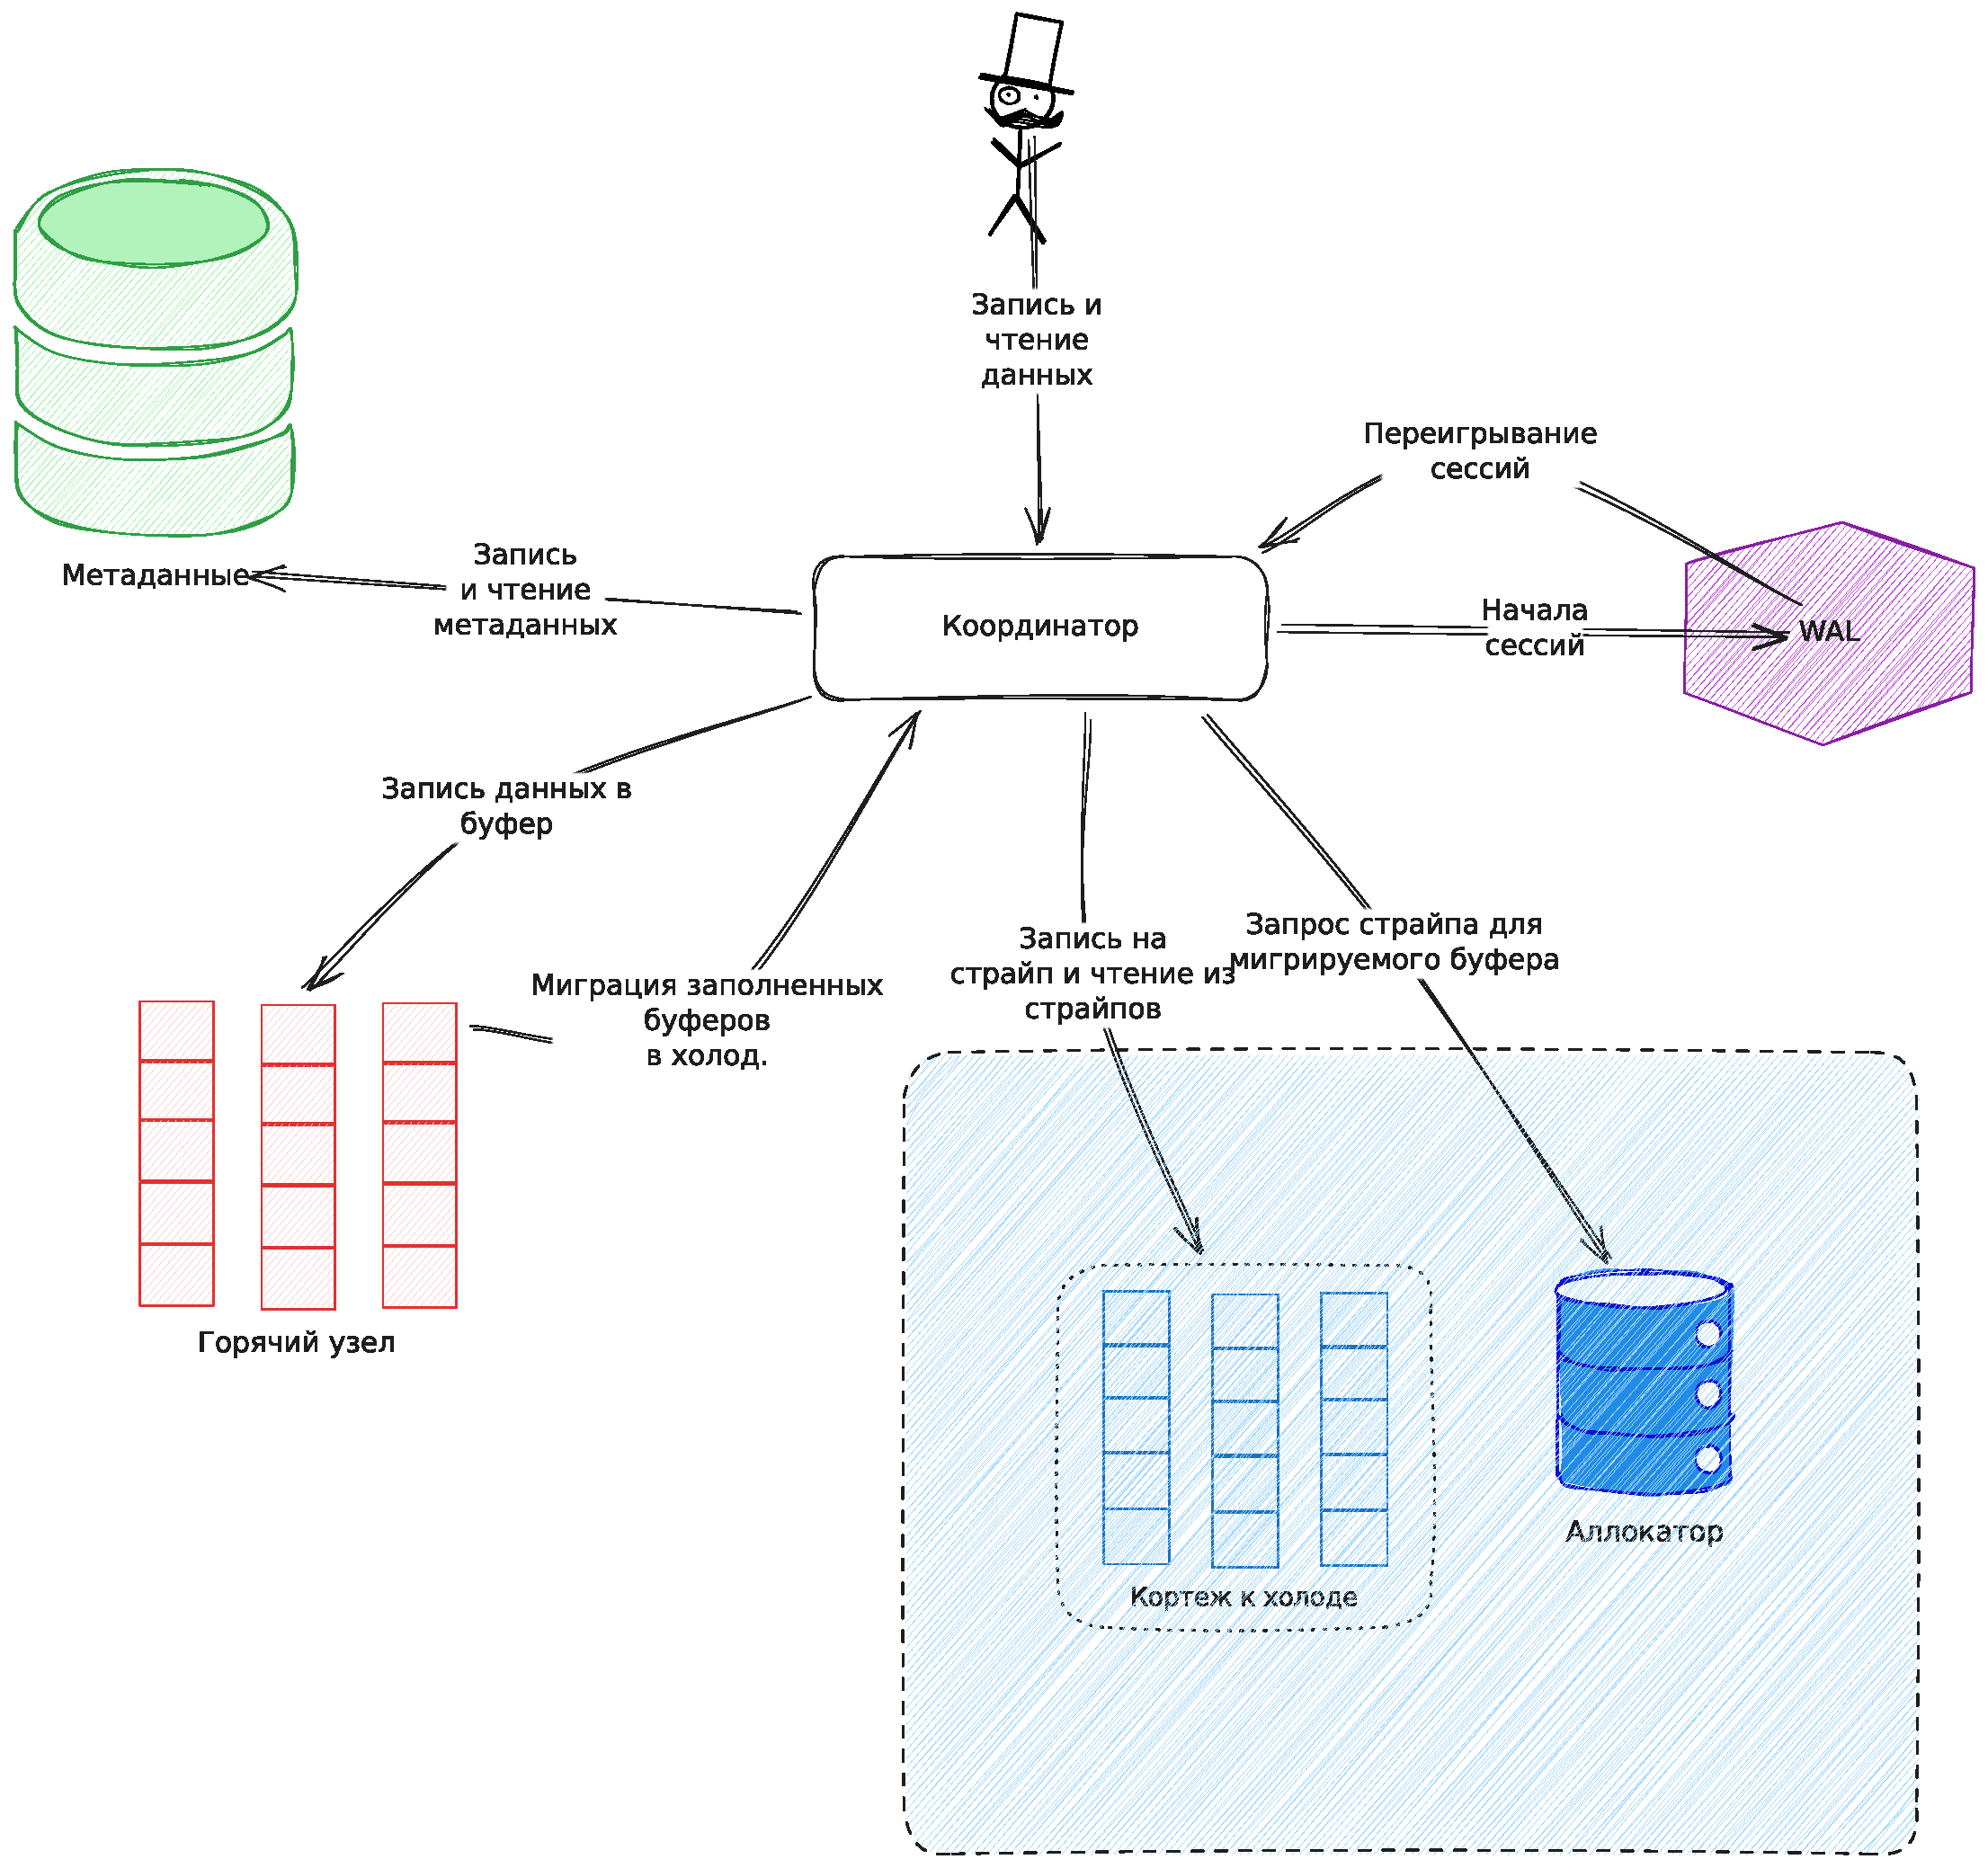
\includegraphics[width=\linewidth]{resources/arch-diagram.pdf}

    \subsection{Вид издалека.}

    Если не углубляться в подробности, схема работы выглядит следующим образом:

    \subsubsection{Запись.}

    \begin{enumerate}
        \item Клиент льёт данные к координатору.
        \item Координатор дробит поток на фрагменты и пишет их жару, а метаданные в БД метаданных.
        \item Координатор возвращает клиенту идентификатор записи.
    \end{enumerate}

    Запись в жару может приводить к периодическим сигналам от неё, приводящим к миграции данных из жары в холод:

    \begin{enumerate}
        \item Жара сообщает мигратору (может быть и координатором) что буфер готов к переносу.
        \item Мигратор вытаскивает данные из жары, находит свободный страйп в холоде и пишет туда полученные данные, а затем отображает это в метабазе.
    \end{enumerate}

    \subsubsection{Чтение.}

    \begin{enumerate}
        \item Клент спрашивает у координатора данные записи.
        \item Координатор по БД метаданных определяет их расположение и читает из холода и/или жары.
    \end{enumerate}

    \subsection{Создание индексов.}

    Заводится etcd хранящий u128 для record.id, fragment.id, container.id и т.д. При старте координатор спрашивает у этого etcd диапазон для record.id, скажем $2^{20}$ чисел. После этого он выделяет их по-одному.
    Далее, чтобы обеспечить равномерное разделение по шардам, мы используем не прямое значение идентификаторов, а кодированое значение SPECK128(id), которое
    выдаёт хорошее равномерное распределение значений. В качестве альтернативы мы можем добавлять hash(id) в таблицы, но это будет стоить некоторых
    объёмов. Лучше использовать SPECK128.

    \subsection{Дедупликация.}

    Данные фрагмента содержат поля

    \begin{center}
        \begin{tabular}{|Sl|Sc|Sc|Sr|}
            \hline
            CRC64 & Size & CompressionType & Blake3 \\
            \hline
        \end{tabular}
    \end{center}

    \bigskip
    Можно держать коллекцию следующего вида

    \begin{center}
        \begin{tabular}{|Sl|Sc|Sc|Sc|Sc|Sr|}
            \hline
            CRC64 & Size & CompressionType & Blake3 & fragment.id & epoch \\
            \hline
        \end{tabular}
    \end{center}

    \bigskip
    И при записи фрагмента искать уже существующие фрагменты по ней. Если есть, то смотреть на эпоху:

    \begin{itemize}
        \item Если она слишком далеко в прошлом, то не используем, а пишем новый фрагмент и перезаписываем эту запись новой ссылкой.
        \item Иначе данные не пишем, а используем существующий фрагмент.
    \end{itemize}

    Такая процедура на самом деле может приводить к некоторому дублированию данных. Это другой процесс проделывает то же самое одновременно: пишет
    фрагмент и заменяет дедуплицирующую запись. Таким образом, мы получим два фрагменты с идентичным содержимым. Но это больше синтетическая
    проблема. В реальных сценариях такое должно быть крайне нетипичным, а сценарий приводящий к массовому распуханию вообще представляется синтетическим.

    \subsection{Процесс обычной закачки данных.}

    При обычной загрузке данных, когда пользователь загружает известный набор данных, вся запись $R$ делится на фрагменты:

    \[R = \left(F_1, F_2, \dots, F_n\right)\]
    где длины фрагментов строго совпадают вплоть до последнего, который может быть меньше остальных. Т.е., формально,

    \[|F_1| = |F_2| = \dots = |F_{n-1}| \geqslant |F_{n}|\]
    Такое ограничение введено для простоты поддержки чтения с отступом. Можно, конечно, было бы разбивать фрагменты на блоки произвольного размера, но это значительно бы усложнило
    стоимость реализации.

    При отдаче пользователем данных – упрощённо, на самом деле там возня с WAL и последовательность обращений к БД метаданных – виде происходит следующее:

    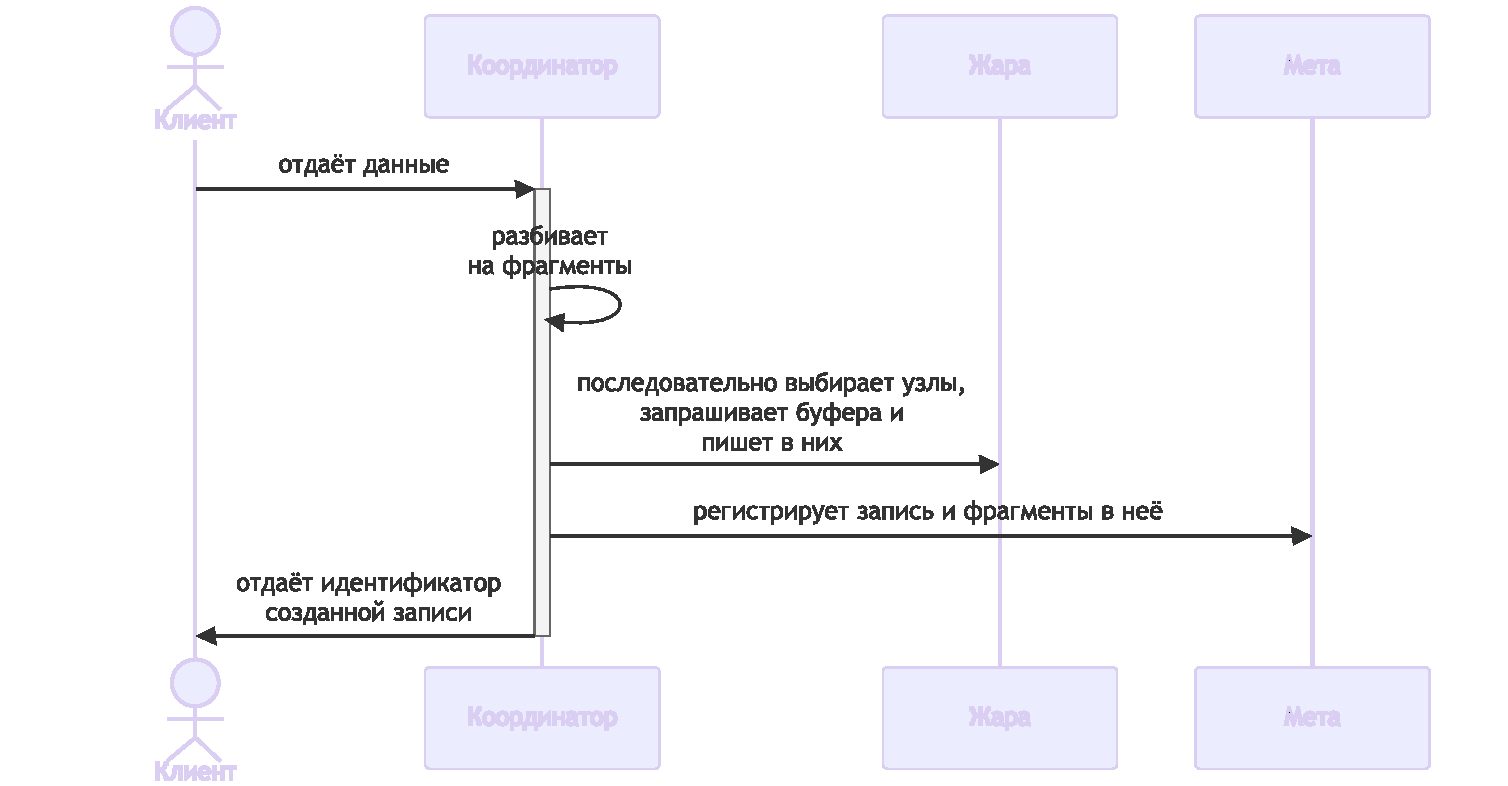
\includegraphics[width=\linewidth]{resources/simple-write}

    В конце материала можно увидеть полную формальную последовательность WritePath с поддержкой фиксации или отката.

    \subsection{Процесс потоковой закачки данных.}

    В это режиме мы берём буфер в жаре во временное владение с подтверждением. И льём туда данные до заполнения. После заполнения запечатываем буфер и ставим задачу на перевоз в холод.
    Из явных отличий от обычной закачки данных нужно отметить ведение фрагмента: содержимое фрагмента в Fragments помечается как \enquote{in progress}, и часть метаданных этого фрагмента (размер и т.п.)
    хранится в метаданных буфера. Это нужно чтобы избежать слишком интенсивных записей в БД метаданных в процессе.

    \subsection{Процесс чтения.}

    Поддерживается полное чтение и чтение с отступом. По пунктам:

    \begin{enumerate}
        \item Получаем record по выданному RecordID.
        \item Читаем идентификаторы фрагментов сканируя Links по ключу (RecordID, <индекс фрагмента>)
        \item Для каждого фрагмента читаем его метаданные из Fragments и находим ContainerID.
        \item Читаем метаданные контейнера из Containers по ContainerID и находим по нему физическое размещение, в холоде ли или в жаре.
        \item Если контейнер в жаре, то делаем запрос на чтение из буфера жары.
        \item Если контейнер в холоде, т.е. адресуется по (TupleID, StripeIndex), то запрашиваем данные кортежа из Tuples и вычисляем по смещению фрагмента в контейнере нужные блоки.
    \end{enumerate}

    \subsection{Миграция из жары в холод.}

    Когда буфер не имеет смысла больше заполнять, т.к. на нём осталось слишком мало свободного места, жара начинает процедуру миграции, обращаясь для этого к \textbf{мигратору.}
    Происходит это по следующей схеме.

    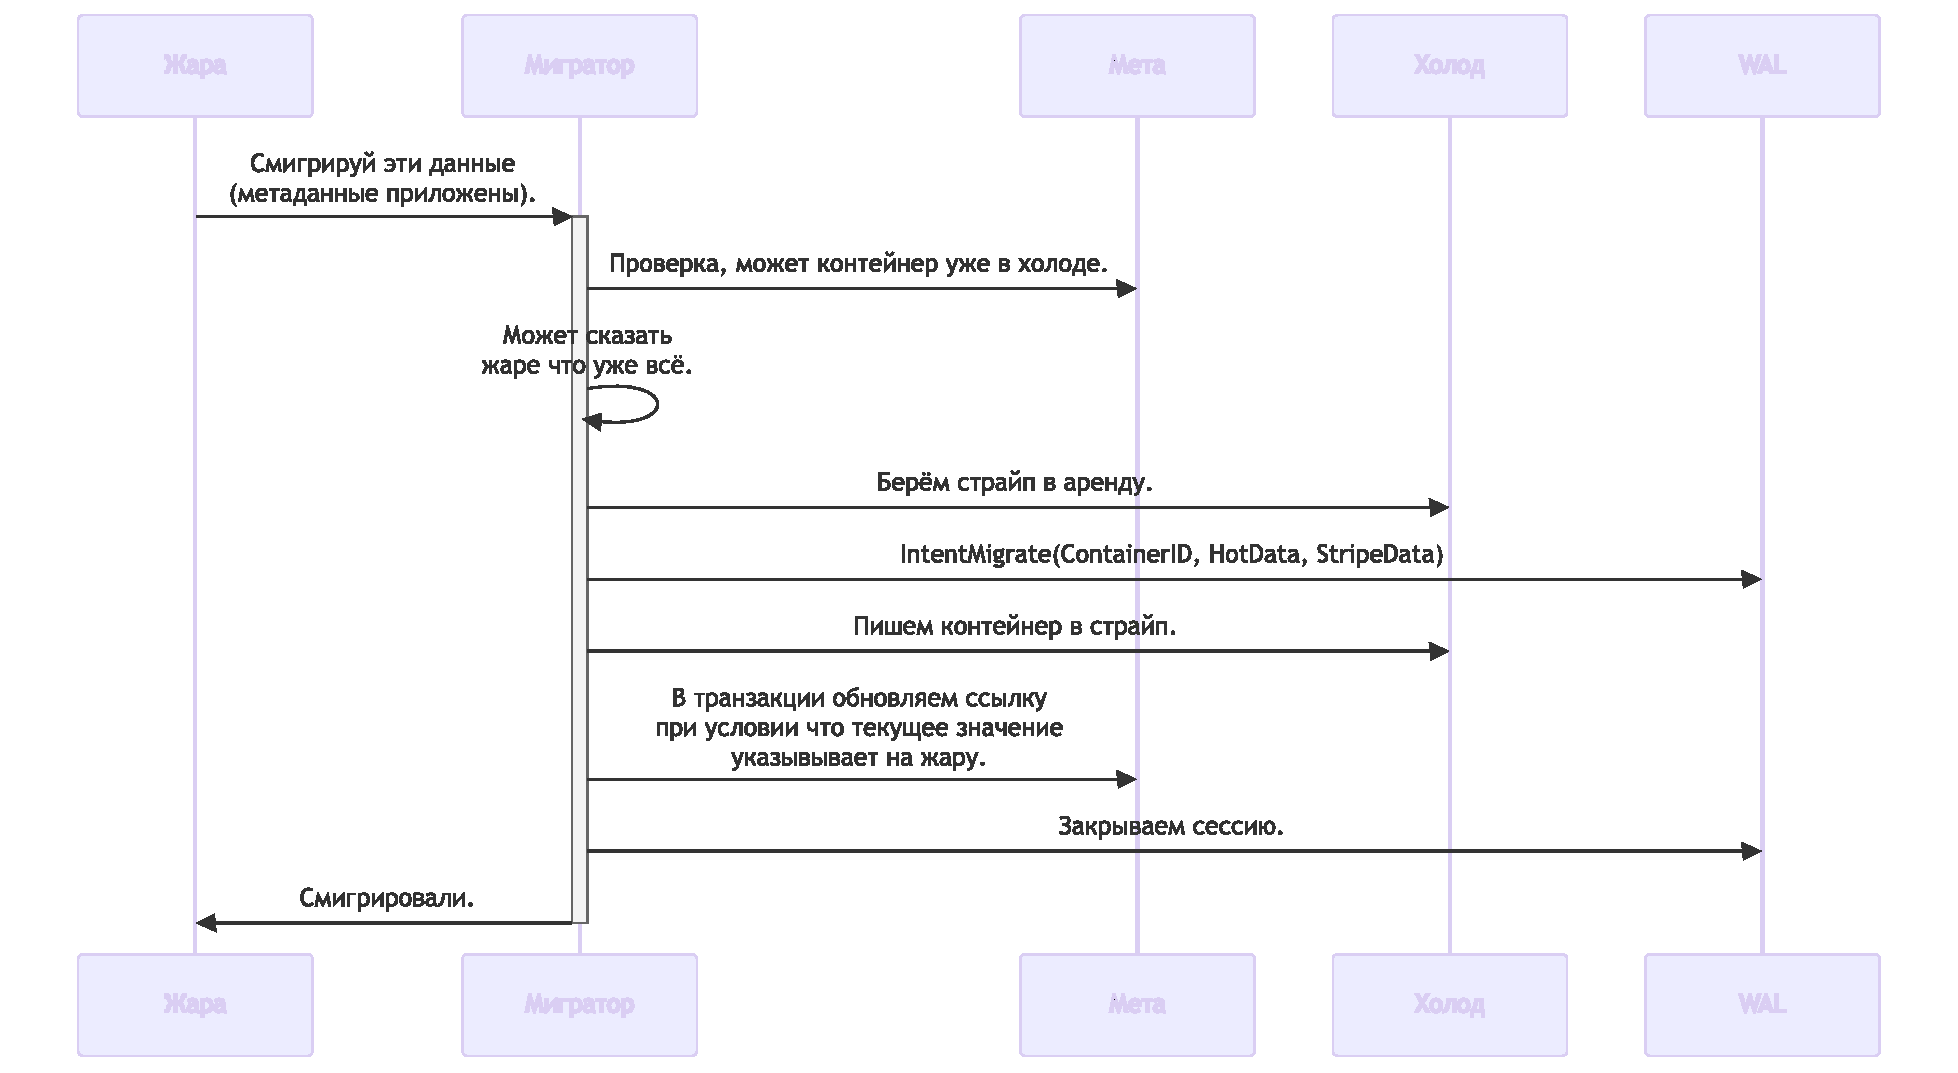
\includegraphics[width=\linewidth]{resources/migration}

    Использование транзакции необходимо чтобы избежать появляение сирот, как указано в этой схеме:

    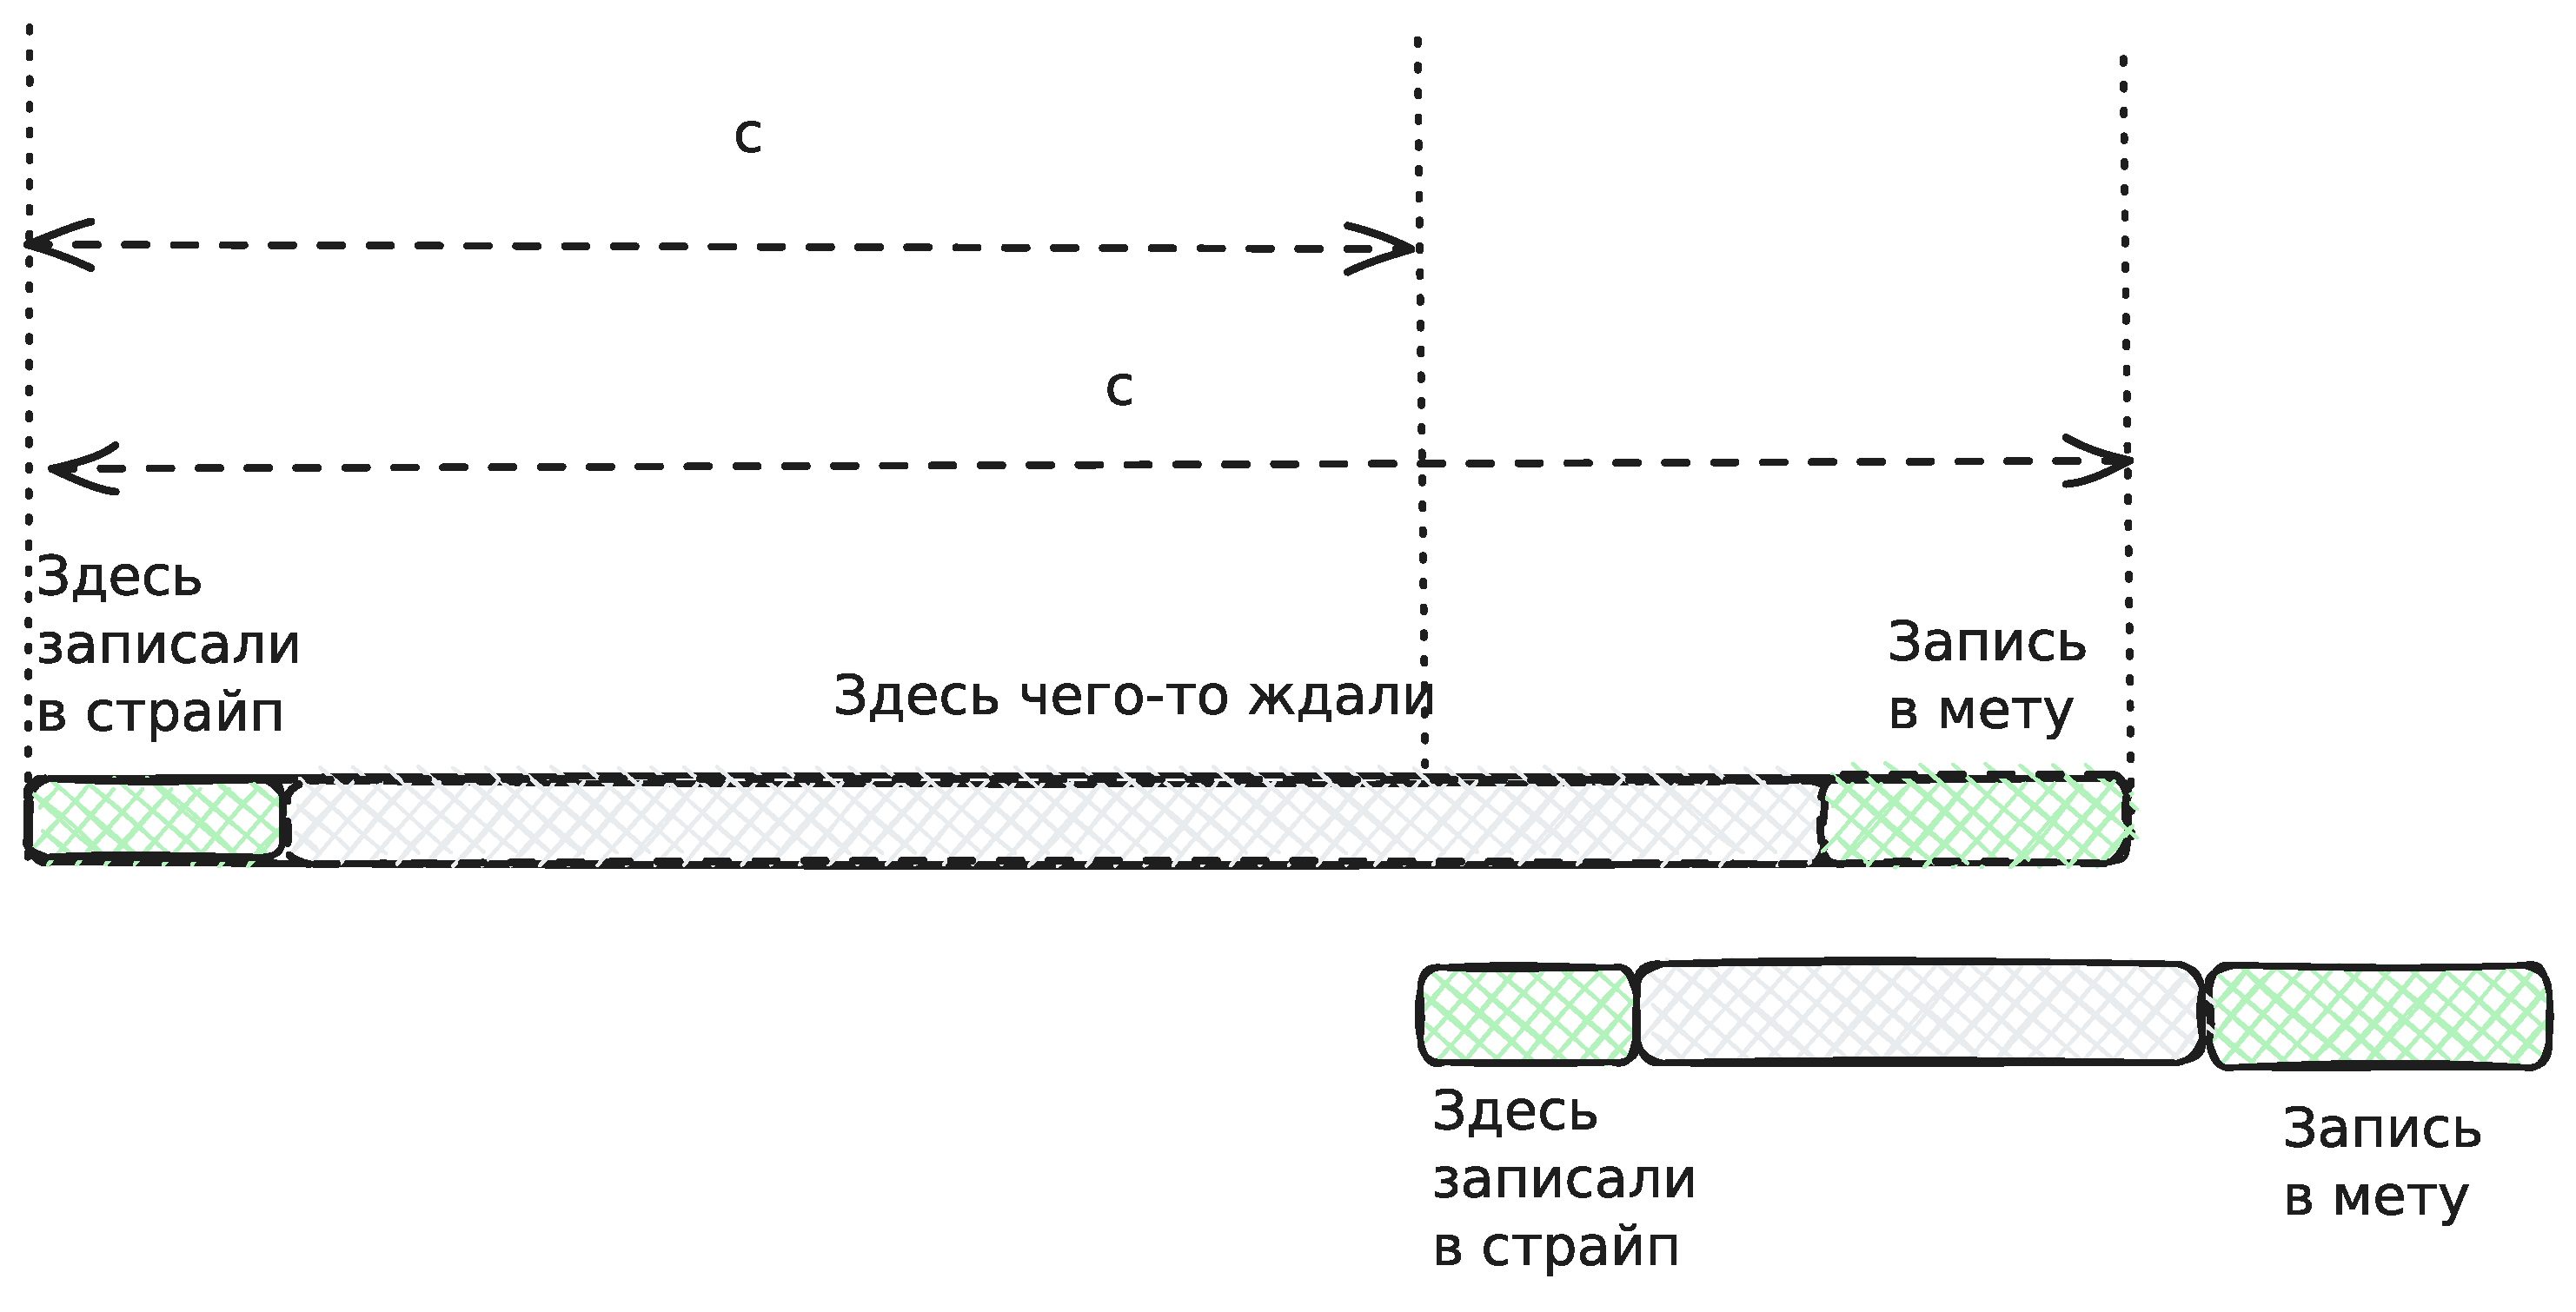
\includegraphics[width=\linewidth]{resources/migration_collision}

    Когда предыдущий процесс может очень сильно затормозить и бысть сочтенным жарой мёртвым. Но остаться в живых и приступить к записи уже после повторной
    попытки миграции. Транзакции здесь не будут слишком обременительными: одна транзакция соответствует записи 64Мб данных. Это смешные для TiKV 32 транзакции при
    2Гб/с записи в систему.

    Данные сохранённые в WAL позволят освободить занятый в текущей сессии страйп, если буфер был перенесён другой миграцией.

    \subsection{Уплотнение данных и GC.}

    \subsubsection{Уплотнение данных на страйпах.}

    Уплотнение страйпов заключается в персборке $N$ страйпов в $M$ страйпов, где $M$ < $N$.
    В метаданных контейнера должны хранится следующие данные: объём незанятого места (не удалось записать фрагмент во время наполнения или фрагмент был удалён – место фрагмента считается свободным)
    и средний размер фрагмента на диске.

    \smallskip
    Наивный алгоритм компактизации выглядит следующим образом:
    \smallskip

    Бежим по записям компактизуемых страйпов и читаем фрагменты, сохраняя в буфере в памяти. В ходе этого процесса, если следующая не лезет
    в буфер целиком (размер буфера = размеру блока в жаре), то выделяем под него страйп и сохраняем там.

    Не наивный чуть посложнее, с переупорядочиванием фрагментов и ведением нескольких буферов за раз. Для того чтобы достичь наилучшего
    заполнения каждого.

    В общем, несложная алгоритмическая задача. Естественно, в процессе регистрируем намерения в WAL, чтобы при потенциальном повторе понимать,
    с какими страйпами мы имеем дело. После успешной перупаковки или сразу после сохранения буфера в страйпе проводим процедуру изменения
    ссылок в Fragments на новые.

    \subsubsection{GC.}
    Это самая сложная тема здесь, пожалуй. Как понятно из всего материала сверху, подчистка ведётся на уровне избавления от фрагментов, которые никем более не используются.
    И она актуальна только для системы с дедупликацией. В случае отключенного дедупа GC не будет представлять никаких сложностей и реализуется путём фонового
    скана кортежей в холодном хранилище, кортеж за кортежом.
    \smallskip
    Фрагменты готовятся к удалению когда на них больше не осталось ссылок в Links. Процедура определения этого факта весьма тяжела если делать напрямую:
    \begin{itemize}
        \item Хранение обратного индекса fragment.id -> (record.id, индекс фрагмента). Работать такое, скорее всего будет, но базке от такого точно будет нелегко.
        Потому что здесь O(1) от Links, а это самая большая коллекция у нас. Но, в принципе, в инсталляциях относительно небольшого размера такое возможно.
        \item Полное сканирование Links. Это тяжело и ненадежно: никто не гарантирует доступность всех шардов во время скана базы. Опять же, в небольших инсталляциях это возможно.
        \item Подсчёт ссылок и хранение времени доступа. Достаточно надёжно: $\operatorname{refcount} \leqslant 0$ и фрагмент не трогался уже длительное время – с большой вероятностью он больше ни на что не указывает.
        Но такой подход требует перезаписей метаданных фрагментов (можно делать раз в сутки: видим что чисталось менее 24 часов назад – не трогаем время последнего чтения).
    \end{itemize}

    Здесь у каждого из вариантов есть существенные недостатки. Можно утверждать, что первые два точно непригодны для \enquote{exascale}. А вот как раз для огромных массивов данных
    можно применить типичный для этого \enquote{exascale} подход с офлайн-обработкой. Для этого нужно кидать события создать запись и \enquote{привязать} фрагмент к записи в сторонее хранилище.
    Например, в Clickhouse, или в хранилище использууемое Spark/Flink (на самом деле кидать будем в Kafka или RedPanda, а уже оттуда оно будет подсасываться в Clickhouse).

    \smallskip
    Скажем, если это Clickhouse, то создание записи можно отражать с помощью (datetime, record.id, 1). Удаление – (datetime, record.id, 0). И сделать record.id – первичным ключом в таблице.
    И если использовать какой-нибудь CollapsingMergeTree, то первая запись будет заменена на вторую после добавления последней.

    \smallskip
    Затем мы можем делать LEFT OUTER JOIN с таблицей отражающей Links по record.id при условии флаг = 1. Тогда record.id будет NULL для записей в Links, если
    запись была удалена. И тогда мы можем пометить такие фрагменты как предназначенные для удаления. Точнее, предлагается подход с \enquote{даунгрейдом} фрагмента:

    \begin{enumerate}
        \item Созданный фрагмент имеет состояние $LIVE$.
        \item Фрагмент в состоянии $LIVE$ попавший под удаление переходит в состояние $DYING$. Оно может быть выражено появлением поля $death\_time$.
        \item Фрагмент в состоянии $DYING$ попавший под удаление на сей раз удаляется, если текущее время больше чем $death\_time$.
    \end{enumerate}

    \smallskip
    Правда, для этого нужно запретить "старые" фрагменты для дедупа. Скажем, если подходящий по хешу фрагмент старше 3-х месяцев, то создавать новый фрагмент, даже если это будет дублем.

    \bigskip
    Такая схема будет полностью рабочей, при условии что рамках записей данные будут лететь как в базу метаданных, так и в "окно" для Clickhouse.
    Скажем, мы записали запись и связь записи с фрагментом в метабазу. После этого сразу выходим, но сессия продолжает работать в рамках сессии
    мы добавляем эти же данные в CH. В случае неудачи записи сессия отправляется на повтор и мы снова пробуем добавить эти данные.

    \subsubsection{Коллизии переупаковки и GC.}

    В описанных выше идеях не были упомянуты возможные коллизии. Так, например, две процедуры уплотнения могут взять один и тот же контейнер и переместить его \enquote{живое}
    содержимое, естественно по разным контейнерам. Что в итоге создаст сироту:
    \begin{enumerate}
        \item Уплотнение номер 1 изменяет для фрагмента $fid$ текущий страйп $A$ на созданный в процессе $B$.
        \item Уплотнение номер 2 делает то же самое, изменяя ссылку из $A$ в $C$.
    \end{enumerate}
    В итоге система теряет любое знание о том, что $B$ содержит фрагмент с данным $fid$, место занимаемое им
    помечено как использование. Мы получили потерю пространства.

    А в случае наложения работы переупаковки и GC возможна коллизия, когда проводится процедура компакции и одновременно довозятся фрагменты на
    удаление. Фрагмент $fid$ переводится в другой страйп и в то же самое время доставка из GC удаляет его, причём
    последовательность выстраивается следующим образом:
    \begin{enumerate}
        \item GC-процесс узнает какой контейнер содержит данный фрагмент.
        \item GC-процесс уменьшает описание свободного места в контейнере.
        \item Переупаковка изменяет ссылку в фрагменте.
        \item GC-процесс удаляет фрагмент из Fragments.
    \end{enumerate}
    В итоге, контейнер содержащий переупакованные данные содержит неправильную информацию о свободном месте.

    В обоих этих случаях можно было бы работать через транзакции, но это может быть слишком дорого. Но всех вариантов коллизий можно избежать,
    если гарантировать, что никакие две процедуры уплотнения не пересекаются. И что никакая текущая процедура уплотнения не пересекается с отражением
    результатов GC. Я предлагаю следующий подход:

    \begin{itemize}
        \item Заводится очередь задач. Она содержит задачи на уплотнение и на удаление. Проще всего сделать это через брокера.
        \item Заводится сервис накидывающий задачи уплотнения в очередь.
        \item Заводится сервис получающий данные от GC и подготавливающий задачи на удаление.
    \end{itemize}

    Исполнитель задачи получивший её вначале пытается взять $lease$ на неё. $lease$ - это запись в TiKV вида $high \rightarrow (low, high)$. Для этого он в выполняет
    в транзакции.

    \begin{enumerate}
        \item Поиск $lease'$ с минимальным $high' \geqslant high$. Если $low' \leqslant low$, то это коллизия. Задача отправляется на переповтор в будущем, а $lease$ не создаётся.
        \item Иначе создаём $lease$ и приступаем к выполнению задачи.
        \item Никаких TTL! Потому что мы можем остаться в ситуации, когда данные перевезены, но метаданные только частично. При разрешении начать работу над незавершенными
        данными могут появиться сироты – занятые контейнеры. На части которых никто не указывает и которые не помечены незанятыми. Операция будет проводиться под WAL-ом и этого достаточно,
        система докатит изменения и в конце снимет аренду.
    \end{enumerate}

    Как ставятся задачи уплотнения: сервис итерируется по регионам, нарезая каждый на куски случайной длины, но находящейся в определенном диапазоне. Если в регионе последний кусок вышел
    меньше минимального, то захватывается поддиапазон следующего региона. При этом, что важно, рассматриваются только поддиапазоны следующего региона с индексами больше чем самый
    большой в диапазоне текущего – это потому что регионы \enquote{под капотом} могут изменяться в процессе. Множество регионов рассматривается как кольцевой буфер, так что \enquote{следующий}
    для послдеднего будет первым регионом в TiKV.

    Сервис-адаптер для GC тем временем читает выхлоп Clickhouse-а, получая идентификаторы фрагментов для \enquote{даунгрейда}. Затем находит регионы в которых лежат контейнеры
    и группирует фрагменты по регионам. Деля, при необходимости, регионы на внутренние диапазоны одинакового размера – так проще всего. Балансируя между количеством задач и размером
    диапазона для $lease$: чем больше задач, тем меньше должна быть длина. Для того чтобы сократить время $lease$ и чтобы сама задача весила поменьше. Проще (и правильнее) всего будет
    на стороне Clickhouse-а упорядочивать выхлоп фрагментов по возврастанию индекса.

    \newpage


    \section{Инварианты системы}

    Данный раздел фиксирует свойства, которые должны оставаться истинными при любых
    сценариях работы системы, включая сбои, повторы WAL-сессий и миграции. Сюда намеренно не включены состояния, существующие
    только в рамках конкретных алгоритмов выполнения (например, $Hot \rightarrow Migrating \rightarrow Cold \rightarrow Compacted$ для контейнера).
    Эти состояния не являются частью модели данных системы и могут изменяться вместе с реализацией.
    Инварианты фиксируют только проверяемые свойства персистентного состояния, достаточные для обеспечения корректности хранения и доступности данных.

    \subsection{Инварианты ссылочной целостности}

    \paragraph{I1. Единственная истина о размещении.}
    Физическое размещение фрагмента определяется исключительно через цепочку:
    \[
        Fragments[fragment.id].container.id \rightarrow Containers[container.id].ref
    \]
    Никакие другие коллекции не содержат авторитетной информации о физическом размещении.

    \paragraph{I2. Контейнер имеет ровно одно размещение.}
    Для любого $container.id$ значение $ref$ принадлежит одному из двух состояний:
    \[
        ref \in \{ Hot(hot.id, block.index),\; Tuple(tuple.id, stripe.index) \}
    \]
    Промежуточные или двойные состояния в метаданных запрещены. $ref$ ссылается на кортеж и страйп
    существующий в коллекции $Tuples$ и битмапе аллокатора.

    \paragraph{I4. Полнота записи single определяется идентификатором фрагмента в Records.}
    Состав записи $record.id$ в формате single определяется идентификатором фрагмента в $record.single(fragment_id)$.

    \paragraph{I4. Полнота записи multi определяется только Links.}
    Состав записи $record.id$ определяется исключительно строками:
    \[
        (record.id, fragment.index) \rightarrow fragment.id
    \]
    Коллекция $Records$ не содержит авторитетной информации о составе записи в формате multi.

    \paragraph{I5. Фрагмент является неизменяемым.}
    После фиксации записи поля:
    \[
        (offset,\; size,\; crc64,\; compression,\; blake3)
    \]
    не могут изменяться. Любое изменение содержимого приводит к созданию нового
    $fragment.id$.

    \paragraph{I6. Целостность кортежа}
    Для любого $tuple.id$ в $Tuples$ количество дисков в массиве $disks$ и их роли должны соответствовать схеме, заявленной в $type$.

    \subsection{Инварианты миграции Hot $\rightarrow$ Cold}

    \paragraph{M1. Завершённость миграции определяется сменой ref.}
    Миграция контейнера считается завершённой только после атомарной замены:
    \[
        Hot(\cdot) \rightarrow Tuple(\cdot)
    \]
    в $Containers.ref$.

    \paragraph{M2. Commit страйпа после смены ref.}
    Страйп считается занятым (Commit) только после:
    \begin{enumerate}
        \item успешной записи всех блоков,
        \item успешной подмены $Containers.ref$.
    \end{enumerate}

    \paragraph{M3. Эксклюзивность записи страйпа.}
    Запись в $(tuple.id, stripe.index)$ допускается только при активном Lease,
    выданном RAFT-аллокатором. Lease на страйп (tuple.id, stripe.index) выдаётся аллокатором только в том случае,
    если конфигурация дисков в кортеже из Tuples позволяет выполнить запись (например, все диски живы и доступны).

    \paragraph{M4. Идемпотентность миграции.}
    Если $Containers.ref$ уже имеет вид $Tuple(\cdot)$, повтор миграции
    обязан завершаться без побочных эффектов.

    \paragraph{M5. Возможность смены ref.}
    Атомарный переход возможен только как $ref\_expected \rightarrow Tuple(\cdot)$, где $ref\_expected$ —
    точное текущее значение $Containers.ref$ ($Hot$ или композитный $Hot$, т.е. не $Cold$).

    \subsection{Инварианты WAL и повторов}

    \paragraph{W1. Все многошаговые операции выполняются через WAL.}
    Любая операция, затрагивающая более одного домена
    (жара, холод, мета), должна выполняться внутри WAL-сессии.

    \paragraph{W2. Повтор не порождает дубликатов.}
    Повтор WAL-сессии не должен создавать дополнительных ссылок,
    страйпов или контейнеров. Повторная операция либо:
    \begin{itemize}
        \item перезаписывает те же значения,
        \item либо обнаруживает завершённое состояние и завершает выполнение.
    \end{itemize}

    \subsection{Инварианты дедупликации и GC}

    \paragraph{D1. Dedup влияет только на выбор fragment.id.}
    Дедупликация не изменяет модель ссылок. Связи записи с фрагментами
    всегда выражаются через $Links$.

    \paragraph{G1. Удаление фрагмента допустимо только при отсутствии ссылок.}
    Фрагмент может быть удалён тогда и только тогда, когда не существует
    строк в $Links$, указывающих на данный $fragment.id$.

    \subsection{Инварианты исполнения}

    \paragraph{E1. Запись в блоки страйпа и в буфер возможна только при живом Lease.}
    Любая операция записи в cold-страйп или в буфер жары допустима только при наличии действительного $lease.id$, выданного соответствующим
    координатором (RAFT-аллокатором или узлом жары). При утрате или истечении Lease операции записи становятся невозможными.

    \subsection*{4.X. Инварианты владения и конкурентного исполнения}

    \paragraph{O1. Единственный владелец диапазона.}
    В каждый момент времени существует не более одного процесса,
    обладающего правом модификации контейнеров диапазона $R$.
    Право определяется действительным $lease.id$, выданным менеджером диапазонов.

    \paragraph{O2. Модификация контейнера только через очередь диапазона.}
    Любая операция, изменяющая состояние контейнера
    (включая перераспределение фрагментов, изменение метрик свободного места,
    результаты компакции или GC),
    выполняется исключительно как задача очереди соответствующего диапазона
    его владельцем.

    \paragraph{Q1. Линейность исполнения задач диапазона.}
    Задачи диапазона исполняются последовательно одним исполнителем.
    Каждая задача имеет уникальный идентификатор $(rangeID, taskID)$.
    Повторная постановка или выполнение задачи не нарушает корректность
    (идемпотентность или обнаружение повторного выполнения).

    \paragraph{Q2. Монотонность прогресса.}
    Для каждого диапазона существует монотонная точка прогресса $ack$.
    Значение $ack$ может изменяться только вперёд.
    Восстановление после перезапуска выполняется путём продолжения
    с последнего зафиксированного $ack$.

    \paragraph{G2. Актуальность инъекции GC.}
    При применении задачи $\mathrm{InjectGC}(container, F)$
    для каждого $f \in F$ действие допустимо только если
    на момент исполнения выполняется
    \[
        \mathrm{Fragments}[f].container\_id = container.
    \]
    В противном случае операция является \emph{no-op}.

    \paragraph{G3. Отсутствие прямой записи GC в контейнеры.}
    Процесс GC не выполняет прямых модификаций структуры контейнеров.
    Он формирует только задачи диапазонов, исполняемые их владельцами.

    \paragraph{M6. Фиксация размещения перед коммитом ресурса.}
    Любой коммит ресурса cold-слоя допустим только после успешного
    атомарного перехода
    \[
        ref_{expected} \rightarrow Tuple(\cdot),
    \]
    выполненного в транзакции.
    При неуспешном переходе ресурс не фиксируется.

    \paragraph{ID1. Каноничность ключевого идентификатора.}
    Во всех структурах, где требуется равномерное распределение,
    используется ключ
    \[
        id_{key} = \mathrm{SPECK}_{128}(id_{raw}),
    \]
    где $\mathrm{SPECK}_{128}$ — биективная перестановка.
    Это обеспечивает статистически равномерное распределение
    контейнеров по диапазонам.


    \newpage


    \section{Дополнительные материалы.}

    \subsection{Полный WritePath для нескольких фрагментов.}

    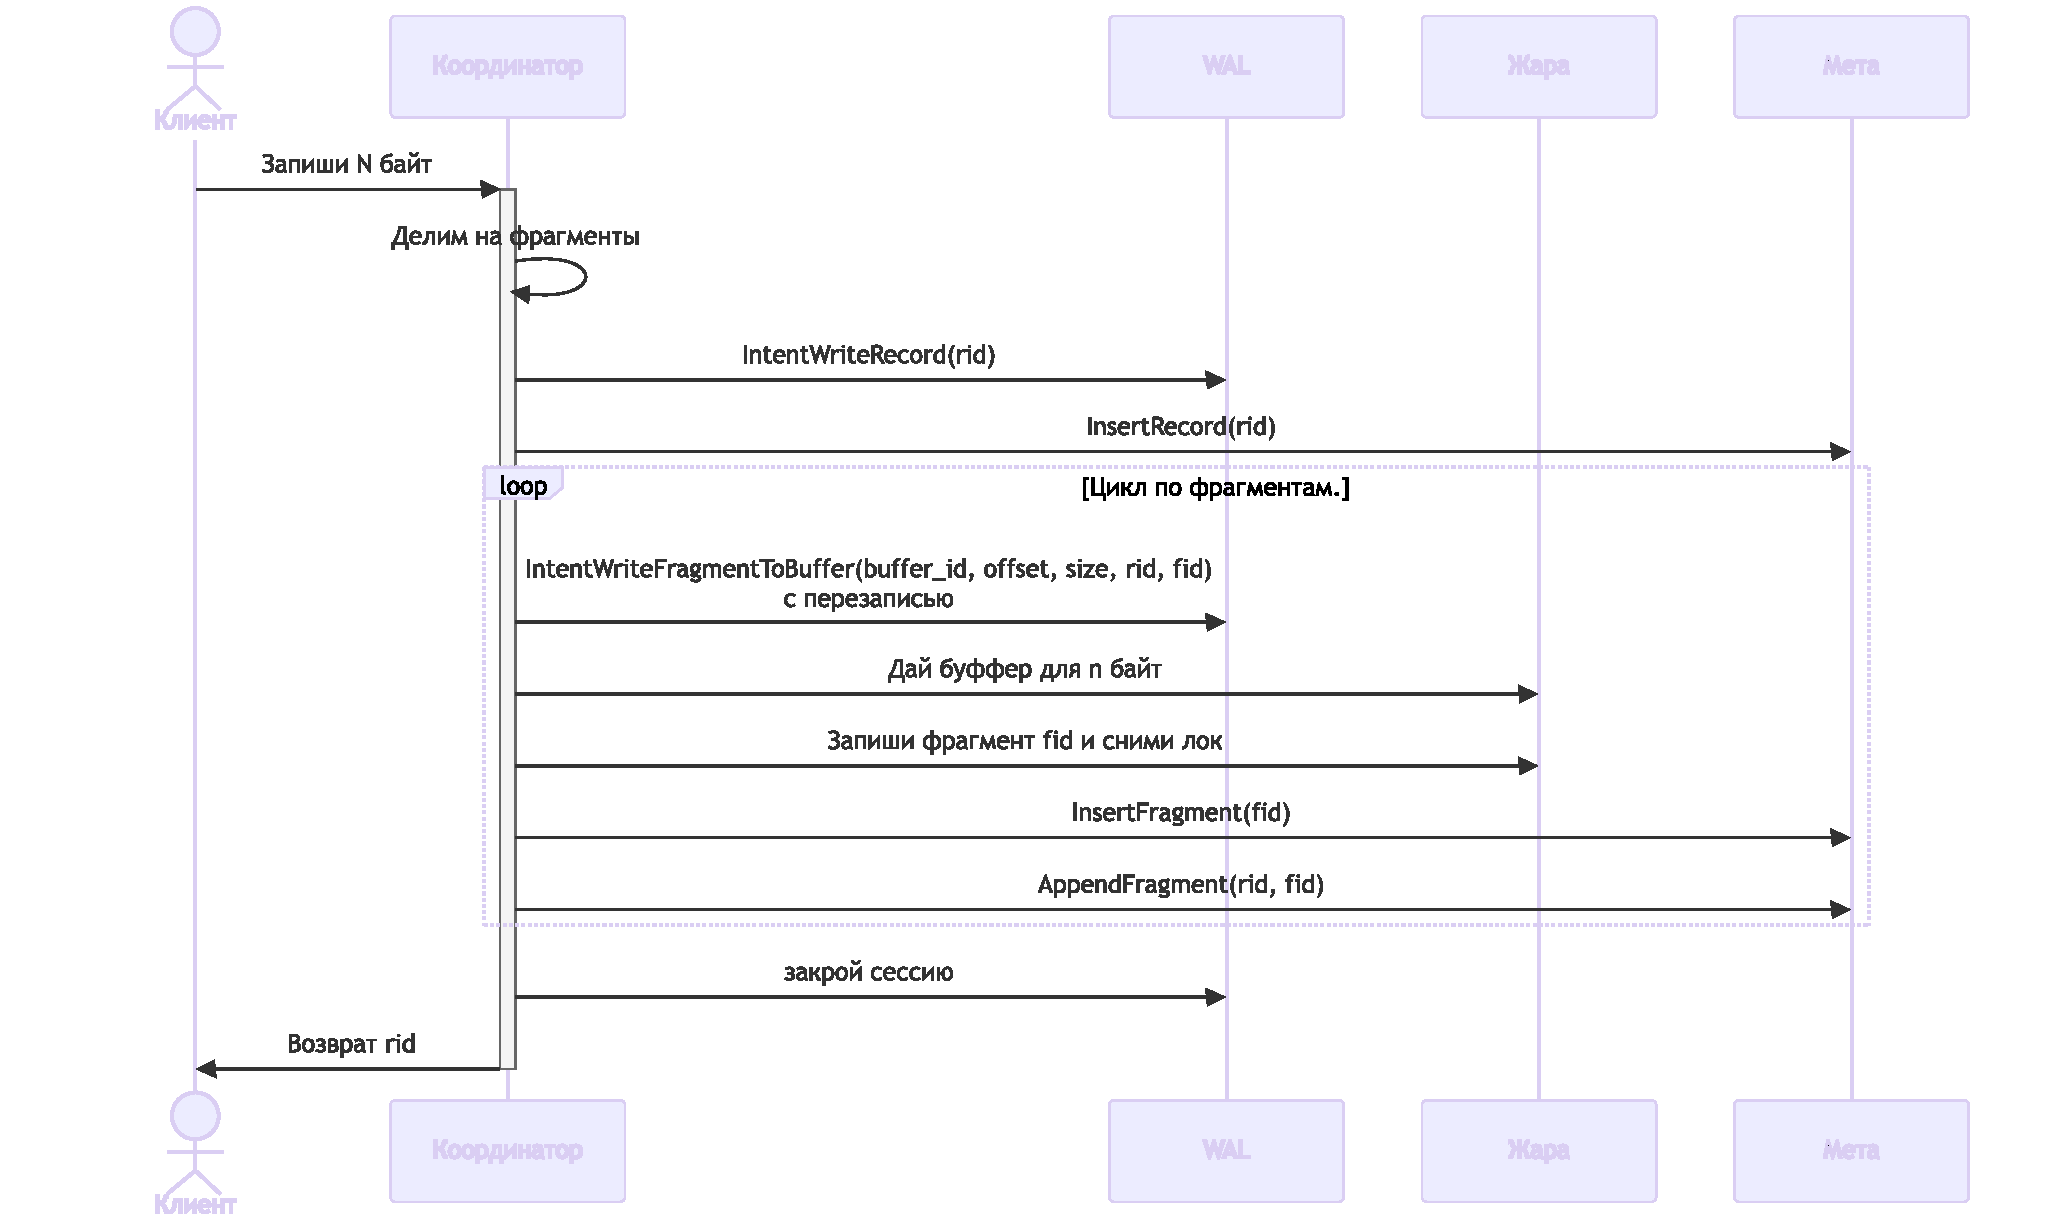
\includegraphics[width=\linewidth]{resources/write-path-multi-hot.pdf}

    Из хорошего здесь то, что операции с БД не должны быть транзакционными, инварианты обеспечиваются WAL-ом и идемпотентностью логики.

    \subsection{Полный MultiWrite.}

    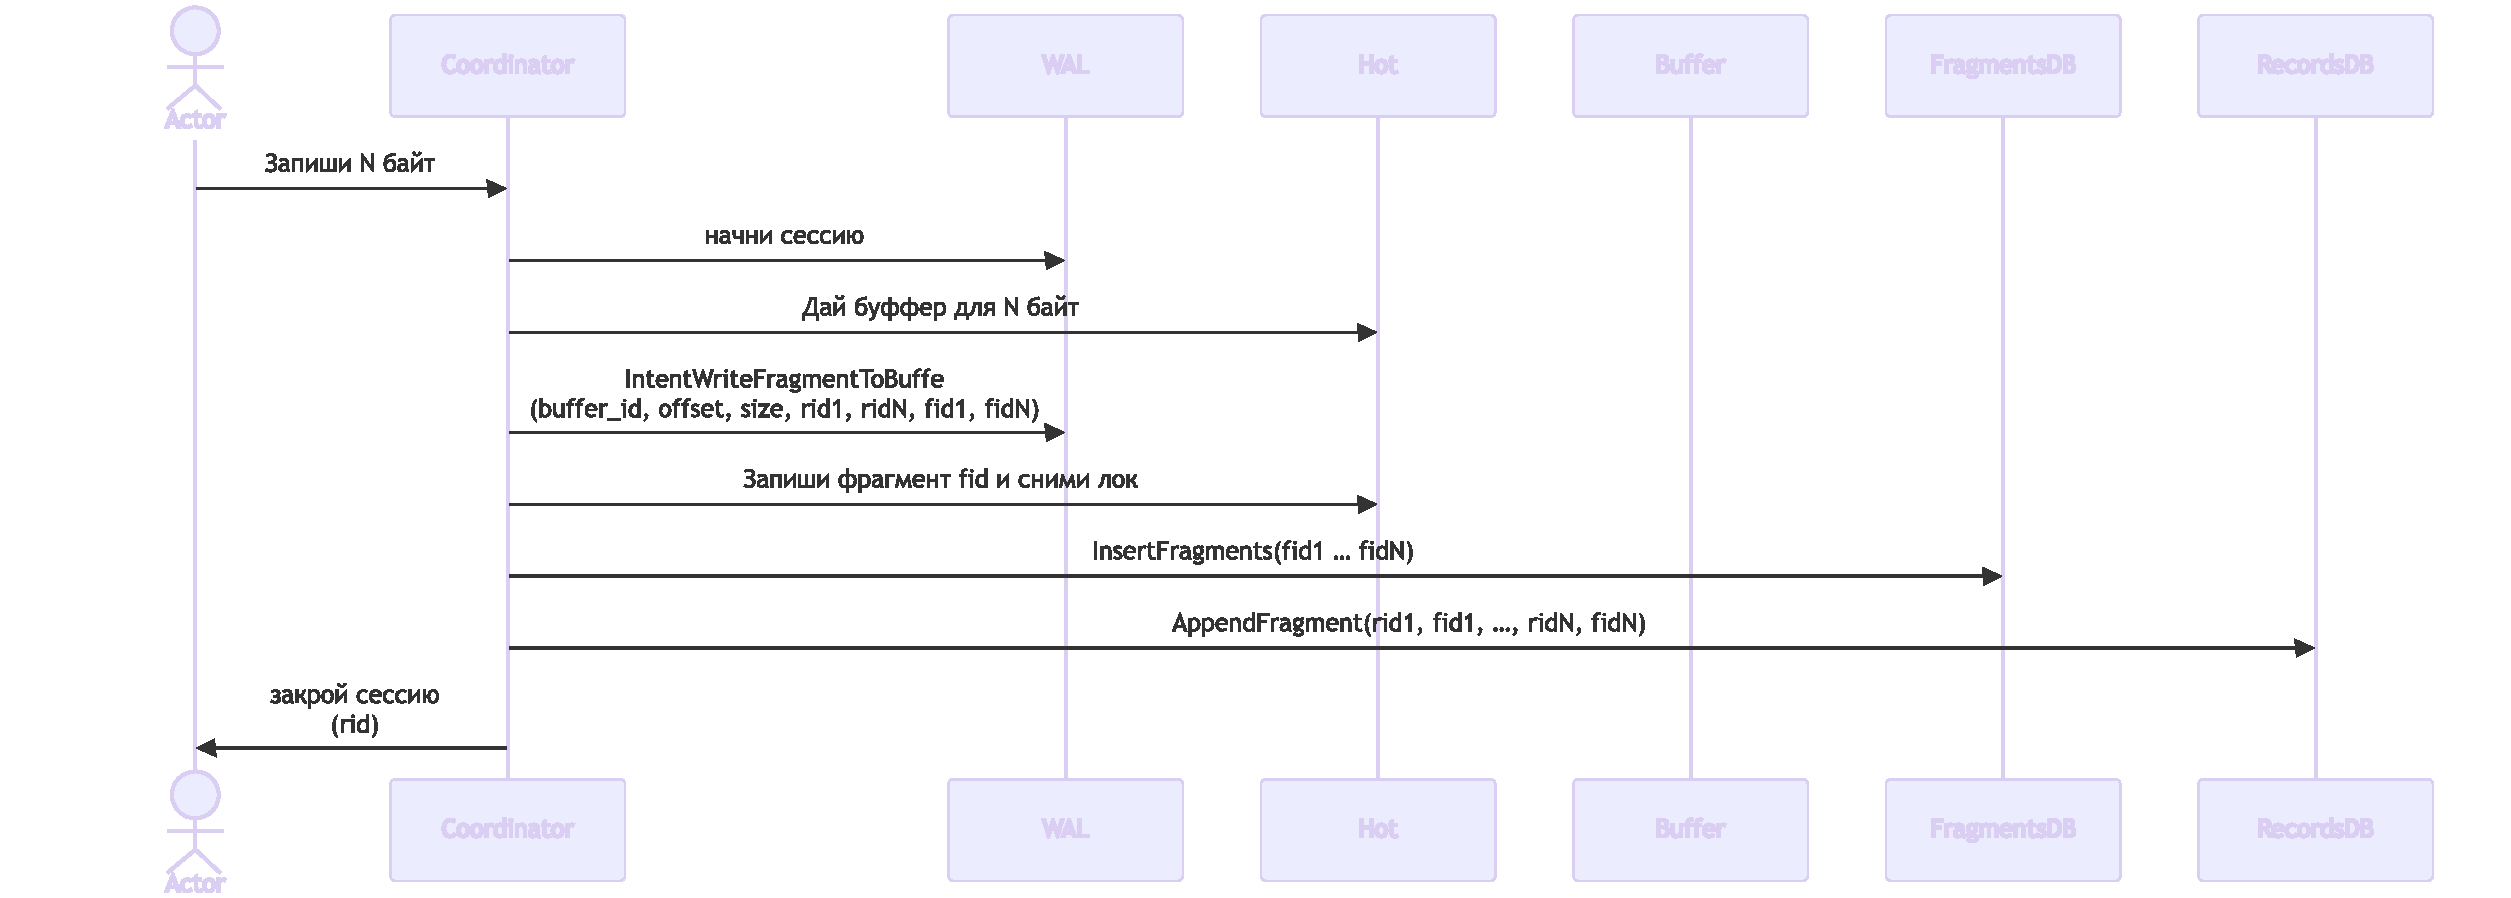
\includegraphics[width=\linewidth]{resources/multi-write.pdf}

    Вставка нескольких фрагментов сразу. Это место критичное для производительности системы при вставке мелких данных. При ней повышенную
    нагрузку получает мета-слой, в который будет лететь куча записей. Схема описанная здесь снимает нагрузку на WAL – использование диапазонов
    (rid1, ridN) и (fid1, fidN) для сохранения намерений в WAL. И нагрузку на хранилише метаданных за счёт использования пакетных записей.

    Обратите внимание, что в качестве rid1 \dots ridN и fid1 \dots fidN использованы "оригиналы" идентификаторов, а не их SPECK128 значения. Как раз для
    того, чтобы мочь использовать диапазонную нотацию, а не перечисления. В случае ошибок в сессии разбор будет вестись уже с преобразованными значениями,
    естественно. Т.е. проверяя ridK из rid1 \dots ridN мы на самом деле проверяем запись с идентификатором SPECK128(ridK).

    \subsection{О реализации WAL с брокером и KV-хранилищем.}

    Реализуется распределенный WAL держащий по логу на сессию. В рамках работы с сессией доступны следующие операции:

    \begin{itemize}
        \item Добавить данные – Append.
        \item Перезаписать данные - Overwrite.
        \item Закрыть сессию.
        \item Отправить сессию на повтор с некоторой задержкой от $T$ секунд.
    \end{itemize}

    Предлагается реализовать эти операции с помощью брокера и KV-хранилища. В качестве брокера предлагается использовать NATS + JetStream.
    В качестве KV всё что угодно. Из персистентных лучше всего подойдут In-Memory хранилища вроде тарантула или Redis. Из хранящих
    на диске хороший кандидат - Aerospike.

    Вариант хранилищ с LSM использующих RocksDB под капотом не подойдёт категорически. Т.к. наша нагрузка подразумевает

    \begin{itemize}
        \item Постоянное создание новых записей, без повтора идентификаторов.
        \item Удаление абсолютного большинства записей в доли секунды.
        \item Большая часть записей переживших те доли секунды всё равно будет удаляться через секунды.
    \end{itemize}

    В этих условиях skip list в RocksDB хранящий таблицу LSM в памяти является крайне неоптимальным вариантом из-за своего
    ленивого характера удалений. Он будет приводить к сильнейшей нагрузке на IO в дальнейшем.

    \subsubsection{Вводные.}

    При заводе сессии координатор получает свежий session\_id, далее просто $id$, о 16 байтах (128 бит). В этих условиях вводим:

    $$K=\operatorname{big\_endian}(id)$$
    $$K'=\operatorname{append}(K, 0)$$

    Т.е. к $K'$ просто прибавили нулевой байт.

    \subsubsection{Работа с KV.}

    При начале работы сразу же запускается фоновый процесс регулярно пишущий unixtime в $K'$, с выставленным TTL = $T$. С периодичностью, скажем,
    в одну секунду. Чаще не нужно. А данные сессии пишутся следующим образом:

    \begin{center}
        \begin{tabular}{|Sl|Sr|}
            \hline
            header & data \\
            \hline
        \end{tabular}
    \end{center}

    Где хидер содержит в т.ч. число повторов совершенных с этой сессией, а данные - последовательность бинарных данных в формате

    \begin{center}
        \begin{tabular}{|Sl|Sc|Sc|Sc|Sc|Sc|Sr|}
            \hline
            varint(len1) & data1 & varint(len2) & data2 & \dots & varint(lenN) & dataN \\
            \hline
        \end{tabular}
    \end{center}

    Все бинарные данные сессии всегда содержатся у координатора. В этих условиях

    \begin{itemize}
        \item Операции Append соответствует добавление к данным сессии нового varint(len(data)) + data и последующая запись всего вместе с
        хидером в значение $K$
        \item Операции Overwrite соответствует удаление всех данных после хидера и добавление нового фрагмента, с последующей записью.
    \end{itemize}

    Когда сессия завершается с успехом, значение $K$ удаляется из БД. Если сессия была неуспешной, просто выходим. Неудача обновления $K'$ считается
    неудачей работы с сессией.

    \subsubsection{Работа с брокером.}

    На определённый топик брокера подписаны все координаторы. Распостранение событий не broadcast, а доставка только одному из подписчиков.

    \smallskip
    В брокер, в этот же топик, летит событие содержащее только $K$, с указанием доставить не ранее чем через $T$.

    \smallskip
    При получении события могут развиваться по следующим сценариям.

    \begin{itemize}
        \item В базе нет записи с ключом $K$. Это означает, что сессия была завершена. Ack.
        \item Значение в $K'$ было слишком недавно. Заказываем передоставку через $T$.
        \item Счётчик повторов в записи $K$ слишком велик. Сообщаем про это в логе, удаляем $K$ и делаем Ack.
        \item Предыдущие пункты не выполнились. Начинаем восстановление сессии запуская обновлялку $K'$, увеличиваем счётчик повторов на один (сразу сохраняя
        новое значение) и начинаем работу по данным записанным в сессии. Далее всё как было описано в пункте \enquote{Работа с KV.}
    \end{itemize}


    \section{Специализированное решение для WAL.}

    Предлагается вариант с Push-Push взаимодействием работающим следующим образом:

    \subsection{Консенсус-узел.}

    Консенсус-узел в WAL состоит из $2n + 1$ машины с налаженными между ними MultiRAFT или аналогичным консенсус-протоколом, с $2n + 1$ внутренним
    RAFT-ом, где каждый хост является лидером одного из них и ведомым для остальных RAFT-ов.

    Каждый хост реализует интерфейс вида

    \begin{lstlisting}
rpc Session(stream SessionReq) returns (stream SessionResp)

type SessionReq oneof {
  Init(clientClass) // Только первый в потоке.
  Append(bytes)
  Overwrite(bytes)
  Close             // Только последний в потоке.
  Repeat(T seconds) // Только последний в потоке.
  Pulse             // Произвольный в потоке.
}
    \end{lstlisting}

    SessionResp содержит подтверждения для проведенных операций, каждый ответ ожидается синхронно.

    Клиент подключается к \textbf{конкретному} хосту такого узла и инициализирует его с помощью Init, затем выполняет последовательность Append/Ovewrite
    и завершает финальным Close/Repeat. При этом в фоне периодически ходит Pulse, так же с подтверждением.

    Активные сессии хранятся в памяти. Сессии оправленные на повтор сохраняются в LSM упорядоченном по времени повтора

    \begin{center}
        \begin{tabular}{|Sl|Sc|Sr|}
            \hline
            repeat\_time & headers & data \\
            \hline
        \end{tabular}
    \end{center}

    Если отвалился клиент, то сессия отправляется на повтор. Если отвалился хост, то бывший ведомый ставшим лидером сессии, немедленно
    отправляет активные сессии полученного RAFT-а на повтор. Повтор сессии начинается по консенсусу.

    \subsection{Клиенты.}

    Сервисы, обеспечивающие обработку повторов сессий, должны реализовывать почти зеркально-симметричный интерфейс

    \begin{lstlisting}
rpc SessionRepeat(stream SessionRepeatReq) returns (stream SessionRepeatResp)
    \end{lstlisting}

    Где SessionRepeatResp выглядит почти в точности как SessionReq, а вот SessionRepeatReq получает новую ветвь, в сравнении с SessionResp:

    \begin{lstlisting}
type SessionRepeatReq oneof {
  Deliver(session_headers, session_data) // Только первый в потоке.
  // Далее в точности как SessionResp.
}
    \end{lstlisting}

    При повторе хост узла определяет класс сервисов на которых нужно вести повтор сессии и подключается для исполнения,
    начиная с доставки данных сессии. Это и есть второй Push в \enquote{Push-Push} схеме.

    \newpage


    \section{Roadmap.}

    \subsection{MVP.}

    \begin{enumerate}
        \item Реализация RAFT-аллокатора.
        \item Реализация сервиса представляющего доступ к дискам машины висящим на JBOD на Go и io\_uring.
        \item Tuples и доведение до ума логики привязки дисков к кортежу (машина может меняться).
        \item Тестирование заливки блоков в "холодный узел".
        \item Реализация выбранного типа хоста горячего хранилища на Go + io\_uring.
        \item Реализация узла горячего хранилища.
        \item Обвязка для WAL.
        \item Сбор всей логики для меты и выбор базы.
        \item Реализация координатора.
    \end{enumerate}

    \subsection{GC.}

    Присмотреть реализацию GC для малых инсталляций и для \enquote{exascale} с Clickhouse через Kafka в сторонке.

    \subsection{Развитие логики.}
    \begin{enumerate}
        \item Группировка кортежей в аллокотаре по типам используемой избыточности. Когда аллокатор рассматривает только
        кортежи сделанные под определенную EC или репликационную схему.
    \end{enumerate}

    \subsection{Оптимизация.}
    \begin{enumerate}
        \item Реализация хоста горячего хранилища с NVMe и NVDIMM на SPDK, выбрать C или Rust.
        \item Реализация узлов с JBOD-ами на Rust с io\_uring.
        \item Замена WAL с костыльного NATS + JetStream на спецализированный Push-Push WAL с мультимастером.
        \item Внедрение архивного слоя, где данные и их метаданные сжимаются в рамках одного контейнера, а TiKV хранит только bloom-фильтры и координаты
        кортежей и страйпов архивного слоя. Разложение данных по страйпам идентично холодному слою, но оперирует меньшими (по P) схемами EC и большими
        размерами страйпов, вроде 1ГиБ вместо 64МиБ. Это позволит снять нагрузку с TiKV, который может начать задыхаться на большом количестве мелкозаписей,
        при котором вес метаданных будет приближаться к весу самих данных.
    \end{enumerate}

    \subsection{Описание механизма \enquote{продолжения}.}

    При стримах у нас может отваливаться буфер. В этом случае можно искать другой буфер в другом месте, и писать в него не сначала, а с позиции обрыва записи на поломанный.
    При переводе склеивать первый и второй буферы по позиции обрыва. Отражая это, естественно, в метаданных.

\end{document}
